\newpage
\section{Конструкторская часть}

Рассмотрим алгоритм Винограда и способы его расспаралеливания.

\subsection{Функциональная модель}

На рисунке \ref{img:idef0} представлена функциональная модель IDEF0 уровня 1.

\begin{figure}[H]
    \center{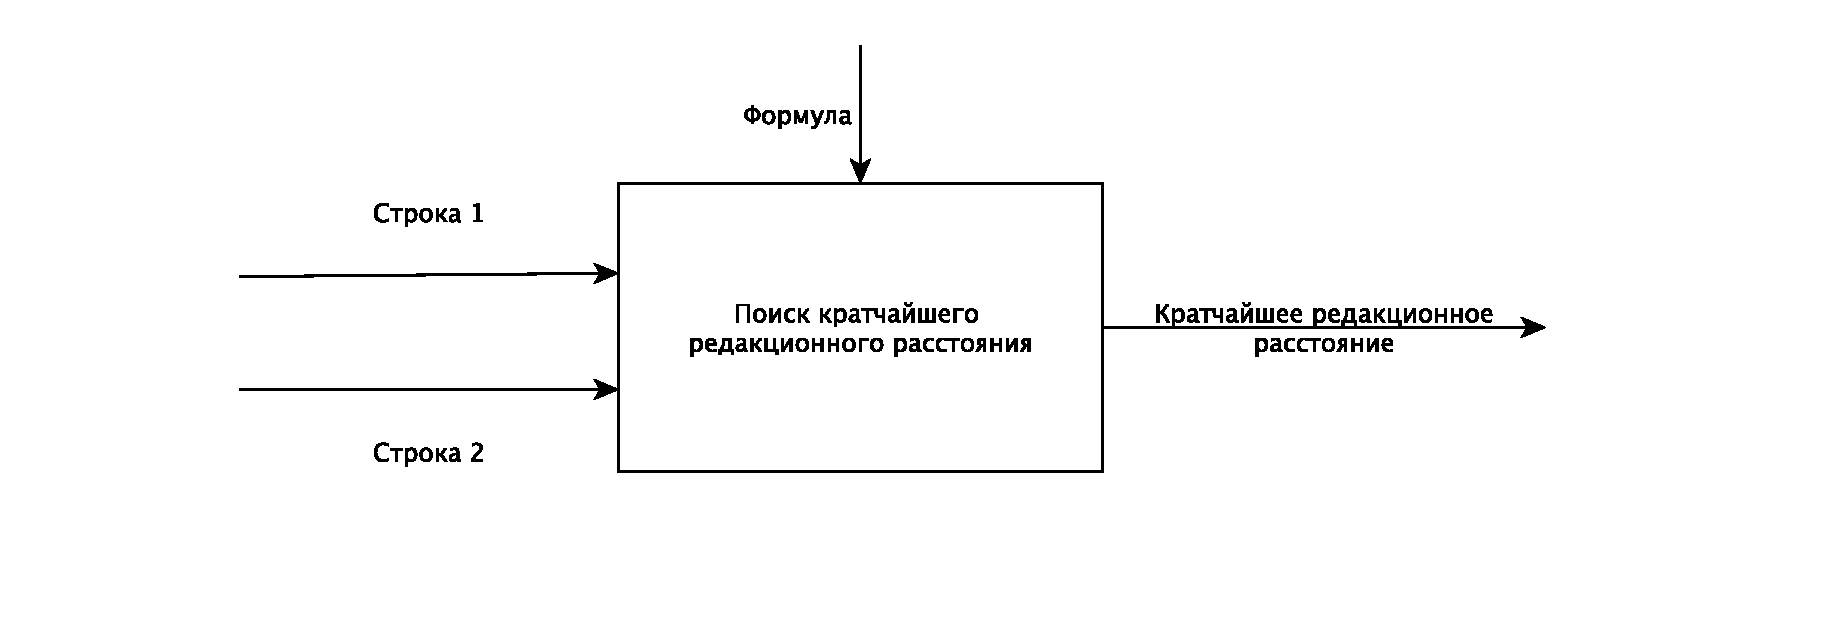
\includegraphics[scale=0.8]{IDEF0}}
    \caption{Функциональная модель IDEF0 уровня 1}
    \label{img:idef0}
\end{figure}

\subsection{Схемы алгоритмов}

На рисунке \ref{img:modvinograd} изображена схема
алгоритма Винограда.

\begin{figure}[H]
    \center{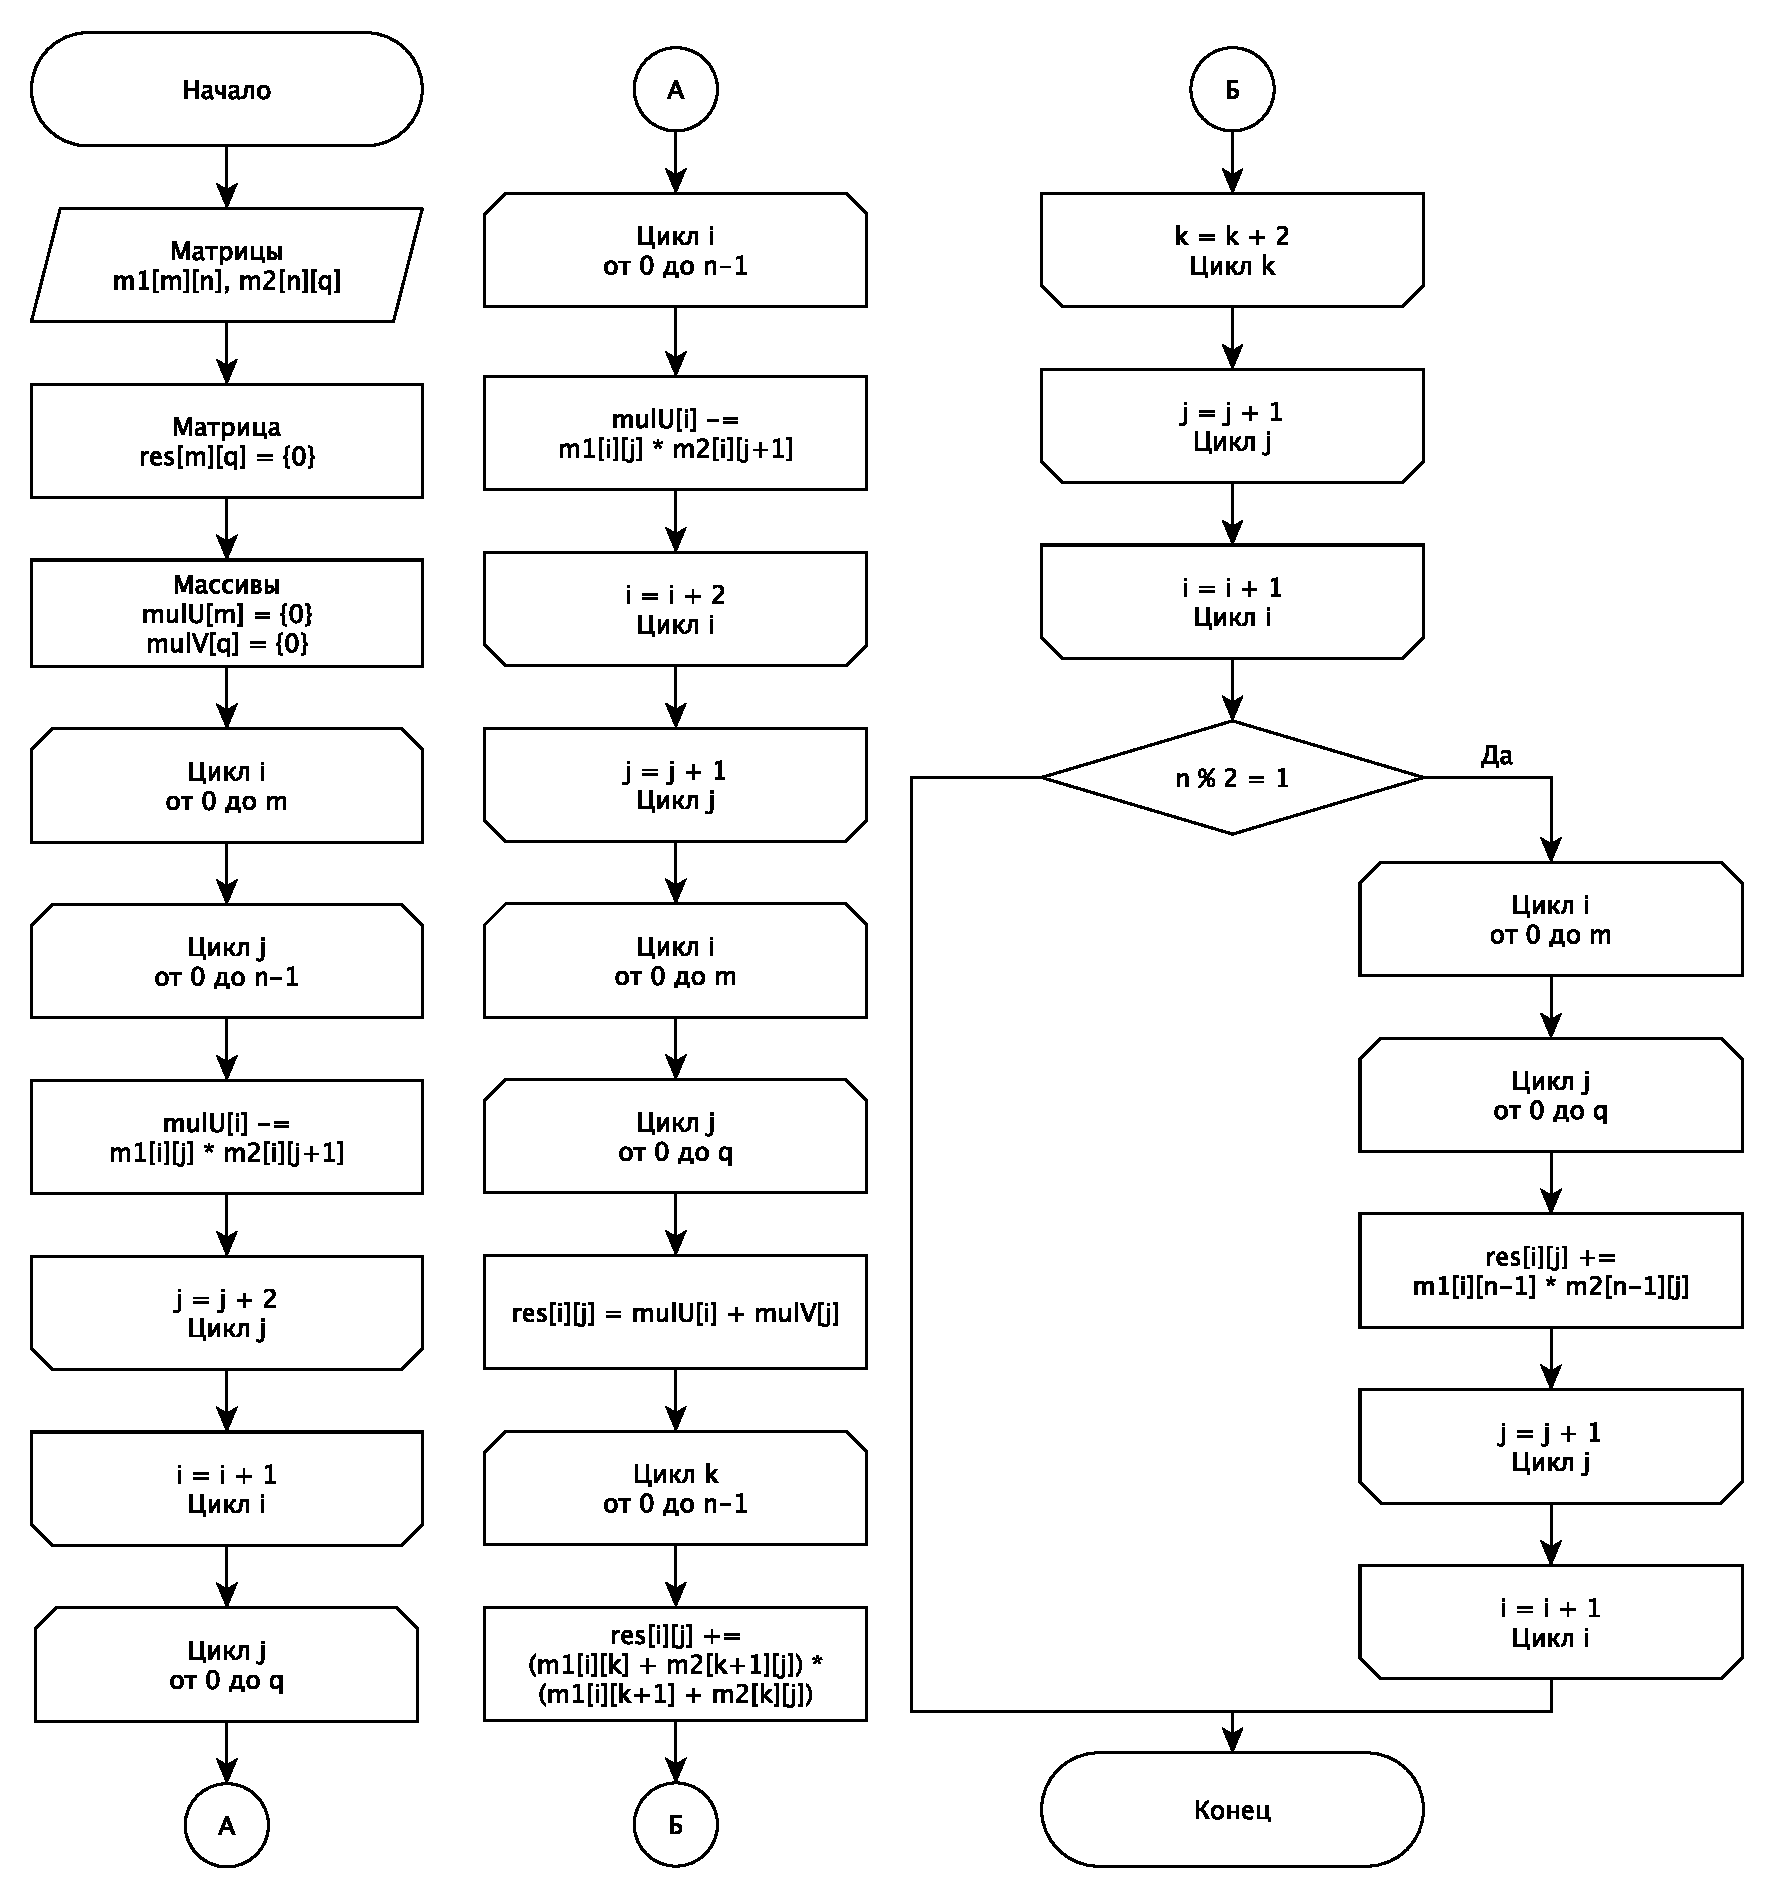
\includegraphics[scale=0.6]{modvinograd}}
    \caption{Схема алгоритма Винограда}
    \label{img:modvinograd}
\end{figure}

На рисунке \ref{img:modvinograd-thread} изображена схема
алгоритма Винограда с возможность распараллеливания вычислений.

\begin{figure}[H]
    \center{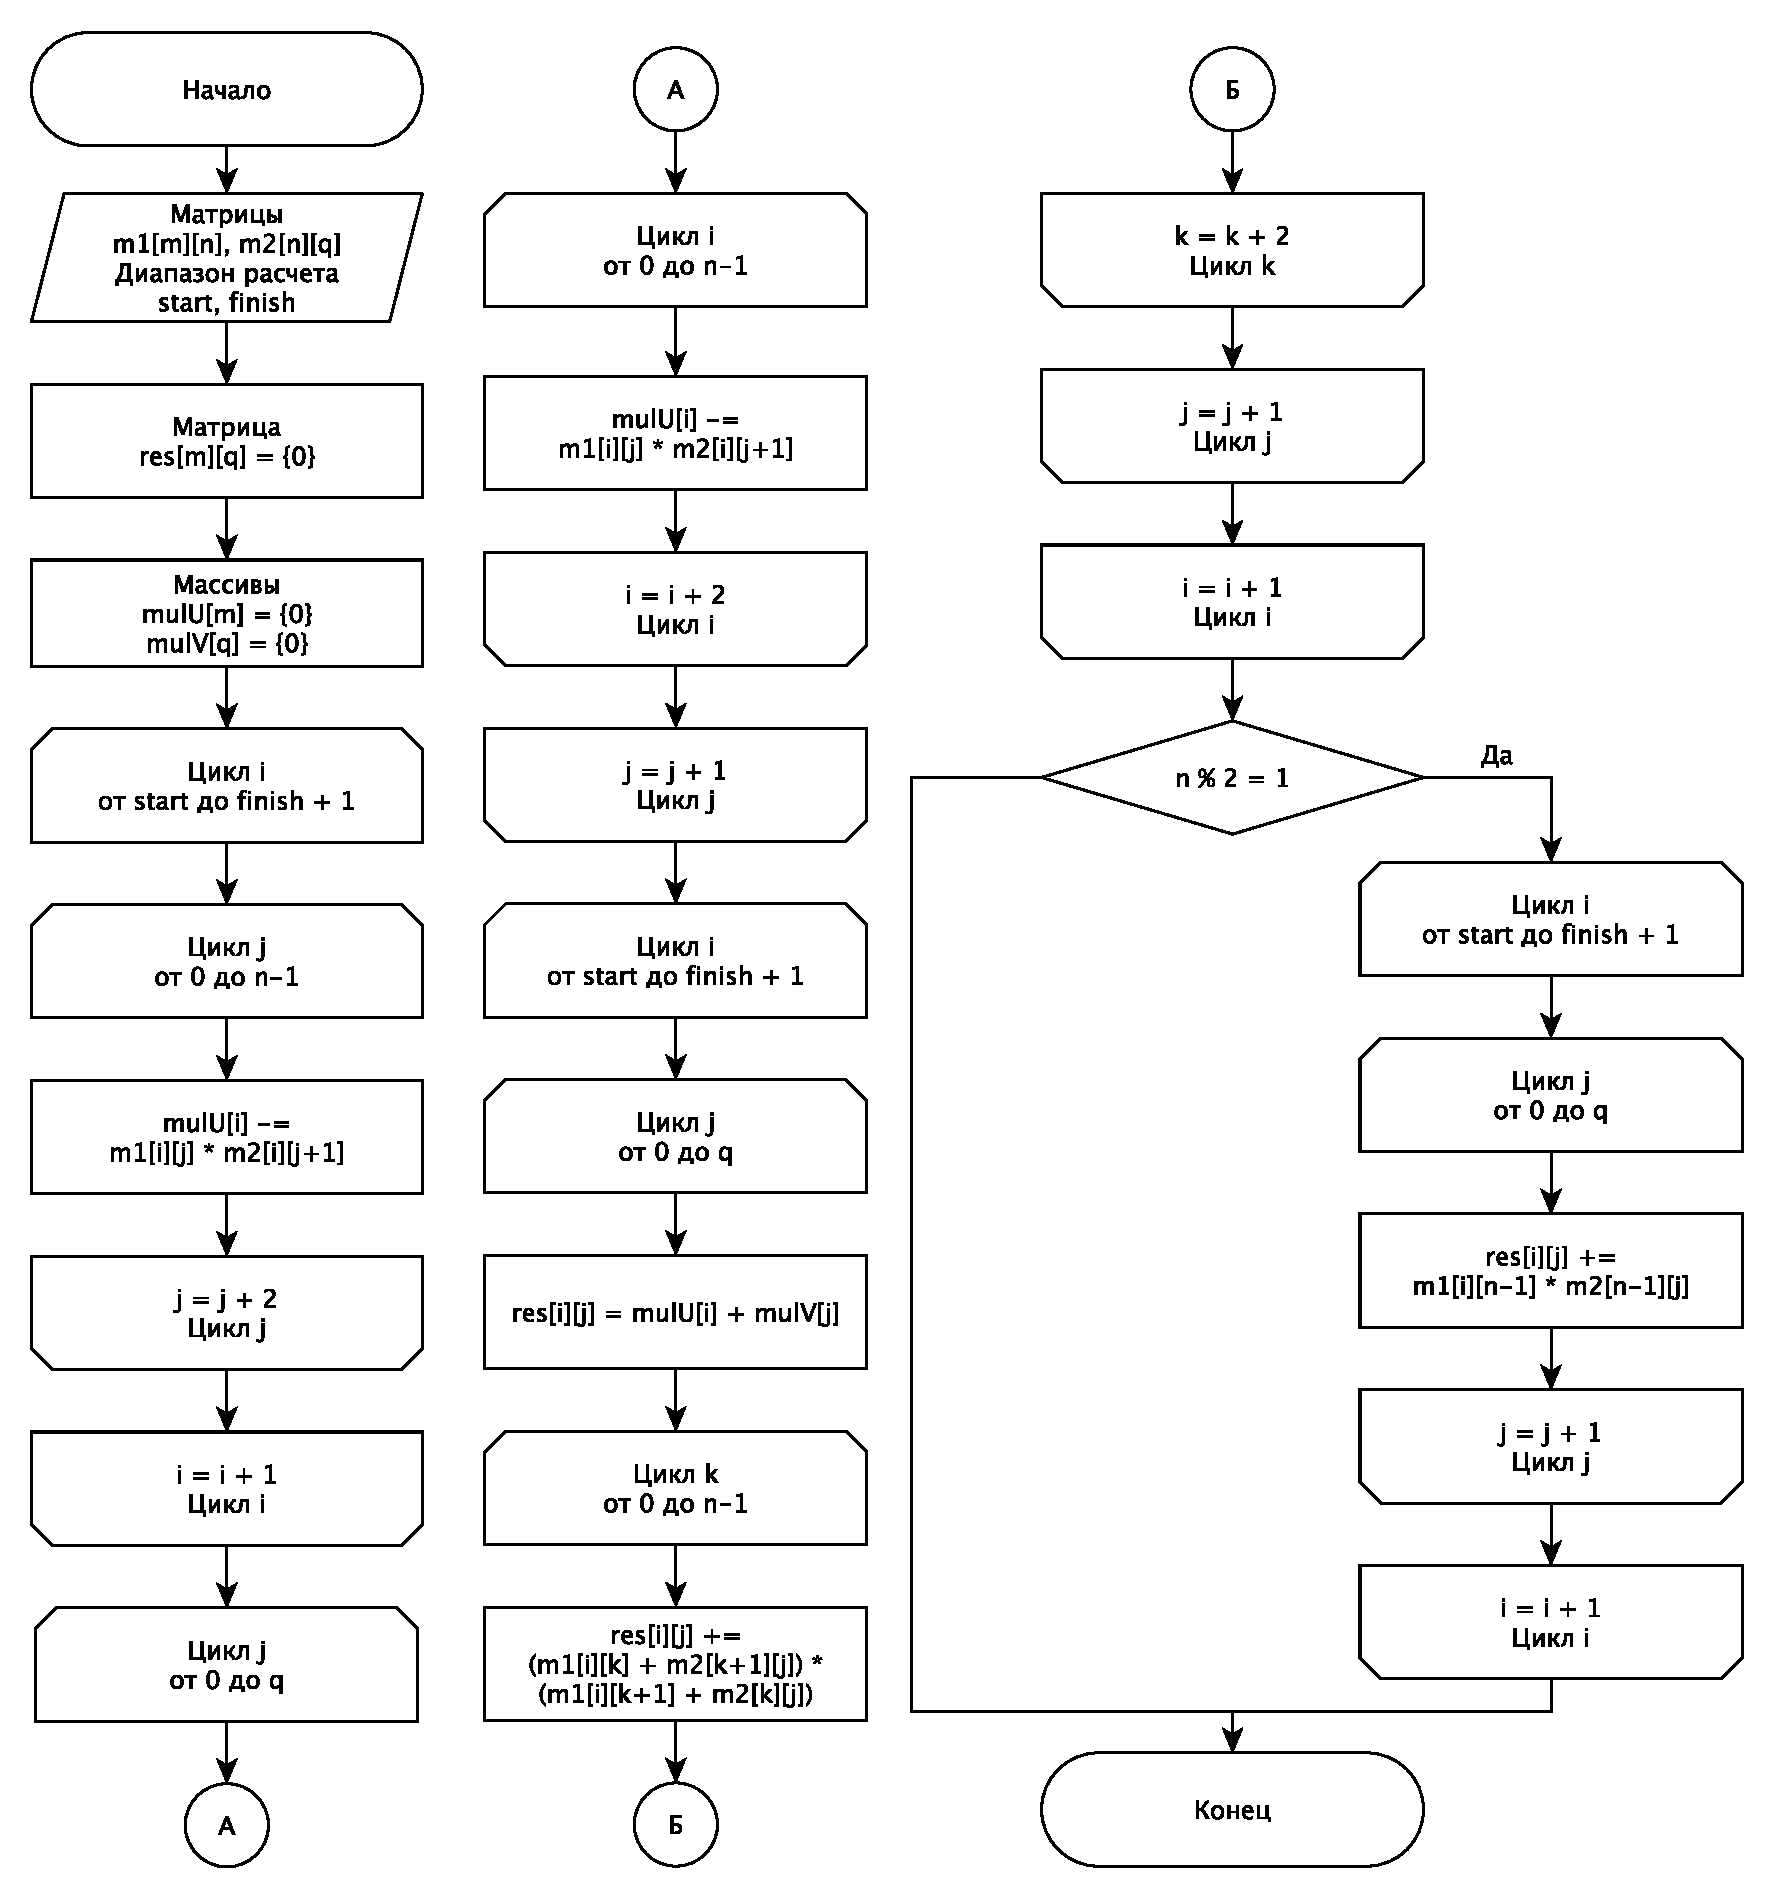
\includegraphics[scale=0.6]{modvinograd_thread}}
    \caption{Схема алгоритма Винограда c возможностью распараллеливания}
    \label{img:modvinograd-thread}
\end{figure}

Распараллеливание вычислений реализовано благодаря добавлению двух новых переменных
{\ttfamily start} и {\ttfamily finish}, которые указывают на диапазон строк, которые
необходимо рассчитать, этот диапазон используется при расчете суммы произведений
{\ttfamily mulU} для строк, а также при расчете результативной матрицы во внешнем цикле, который
отвечает за строки. Передается итоговая матрица с помощью ссылки, что позволяет
одновременно нескольким потокам взаимодействовать с матрицей.

\subsection{Выводы}

Благодаря возможности вычислять каждый элемент результативной матрицы отдельно друг от друга,
удалось разделить вычисления по строчкам, выдавая каждому потоку диапазон строк, в которых
необходимо считать. После выполнения всех потоков и соответственно расчета всех строк матрицы,
получается правильный результат.
